
\section{Headbanger System Design}
\label{sec:design}

\begin{figure}[h]
\centering
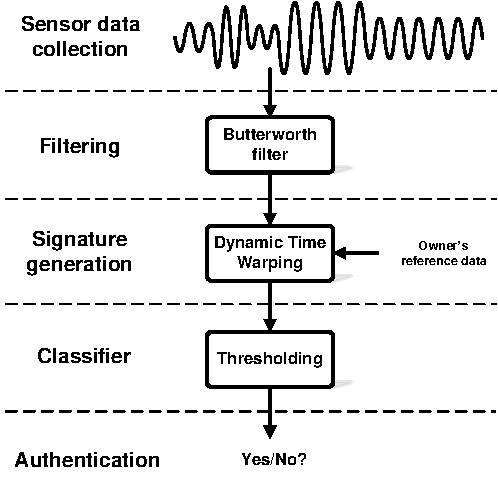
\includegraphics[width=0.95\columnwidth]{../fig/sysarch.eps}
\caption{\systemname~system design flow. The online authentication phase of \systemname~consists of the following steps: (1) sensor data collection in which we collect accelerometer data while users move their head as a response to an audio track played on the glass, (2) filtering in which we apply a Butterworth filtering to smoothen the sensor data for subsequent processing, (3) signature generation in which we calculate the dynamic time warping (DTW) distances between two accelerometer samples as the signature, and (4) classification in which we adopt an adaptive thresholding mechanism to classify the user's head movement, whose result will be used as the authentication result.}
\label{fig:sysarch}
\end{figure}

\begin{figure*}[t]
\begin{center}
\begin{tabular}{ccc}
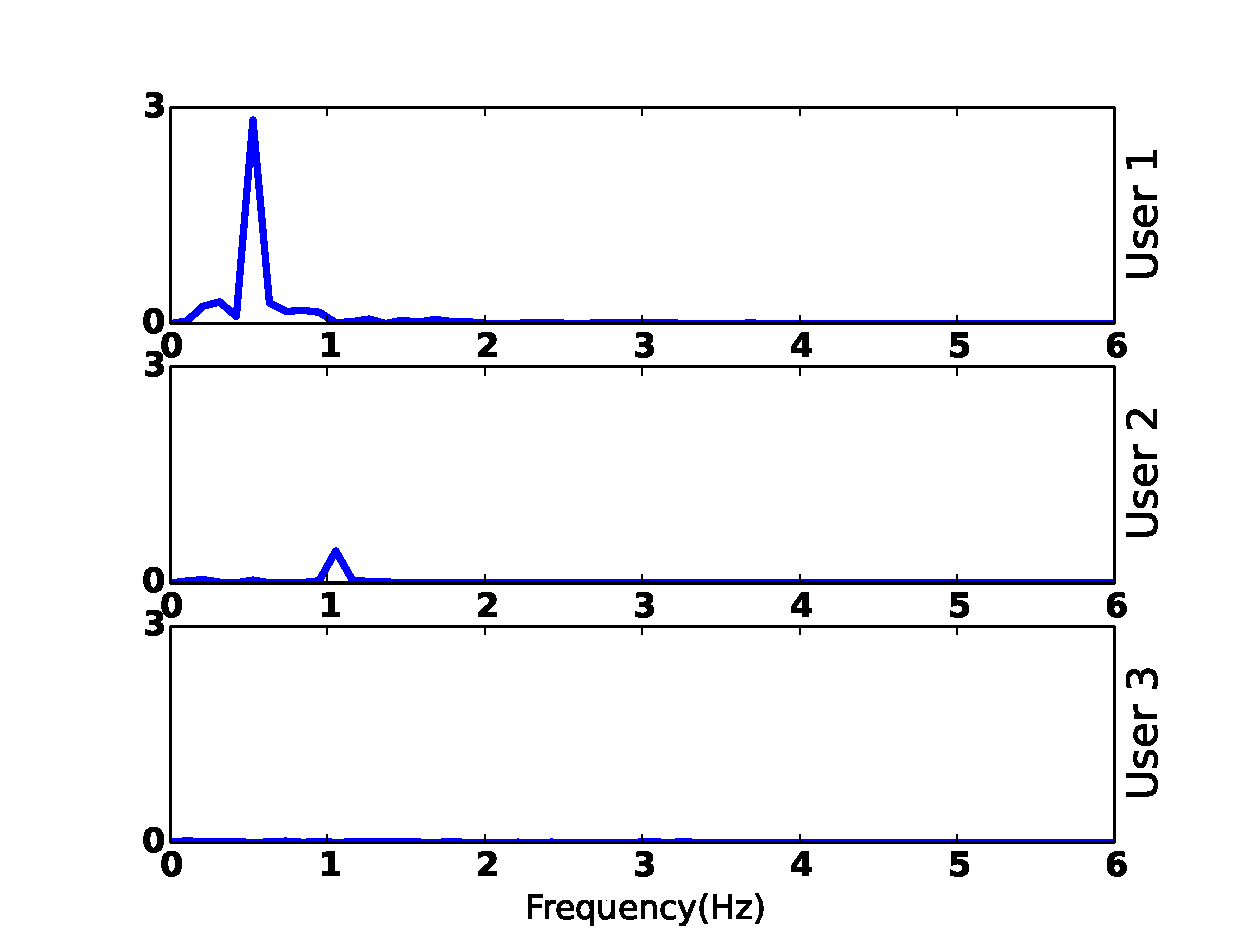
\includegraphics [width=.33\linewidth]{figure/freq_x.eps}&
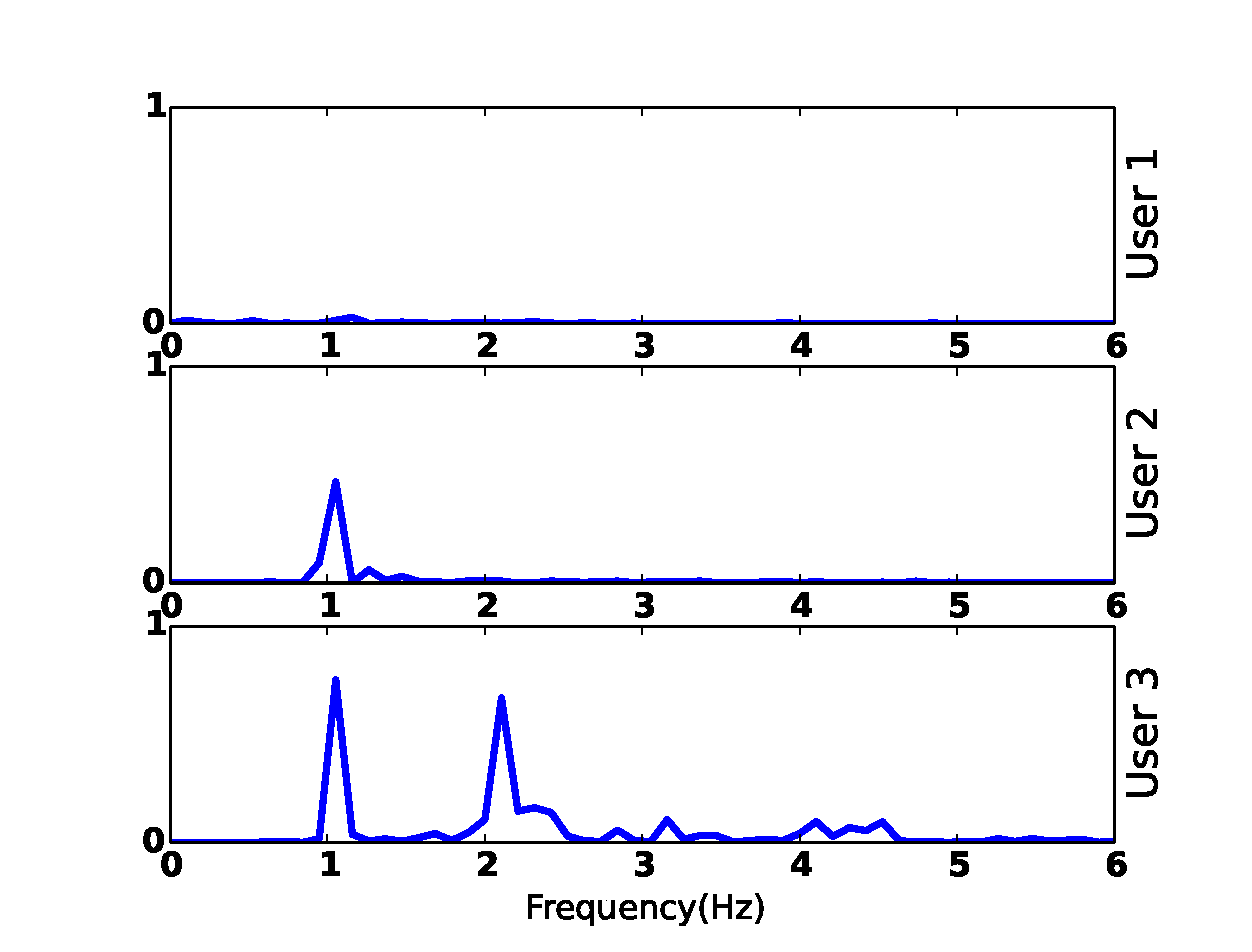
\includegraphics [width=.33\linewidth]{figure/freq_y.eps}&
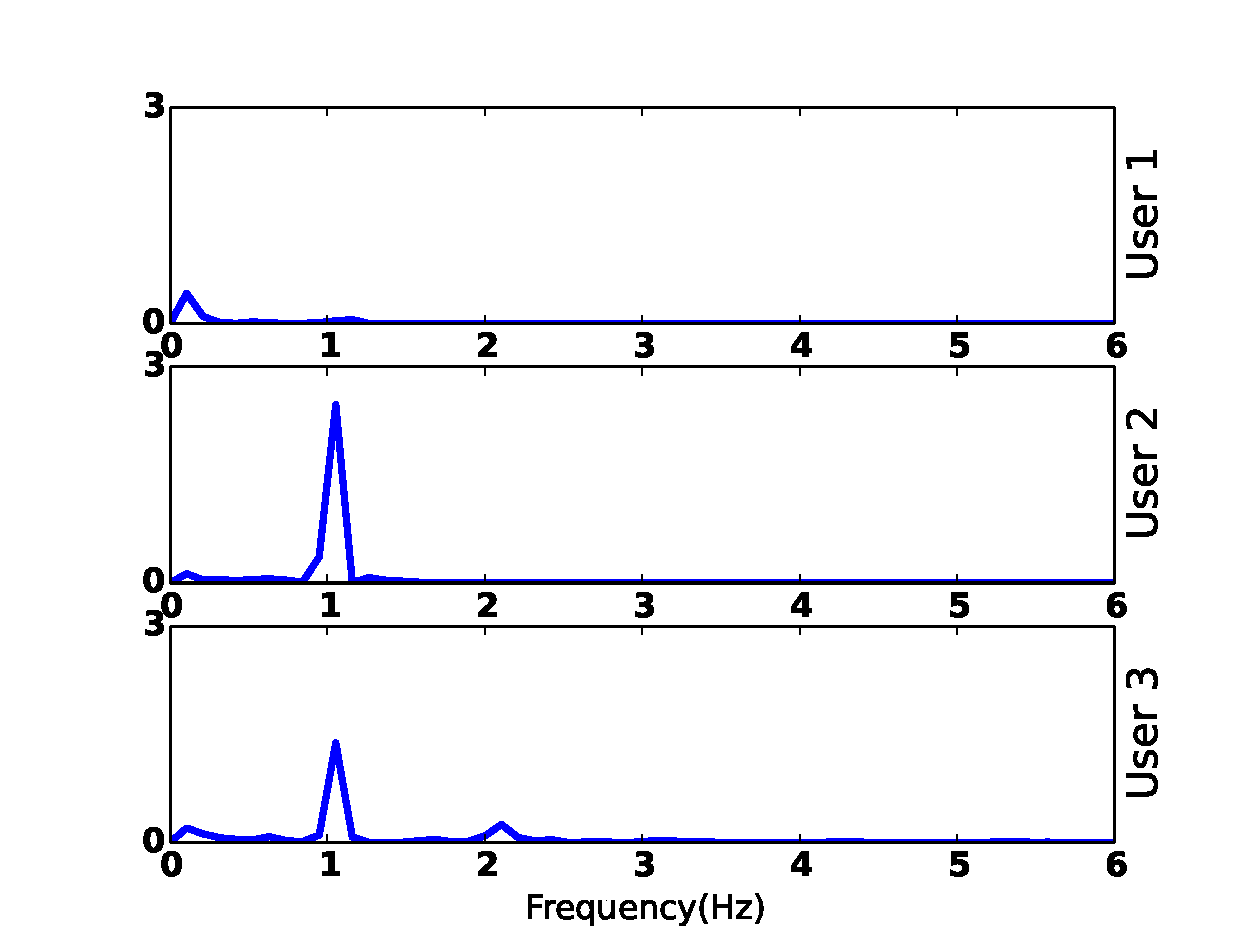
\includegraphics [width=.33\linewidth]{figure/freq_z.eps}\\
(a) X-Axis & (b) Y-Axis & (c) Z-Axis \\
\end{tabular}

\iffalse
\begin{tabular}{cc}
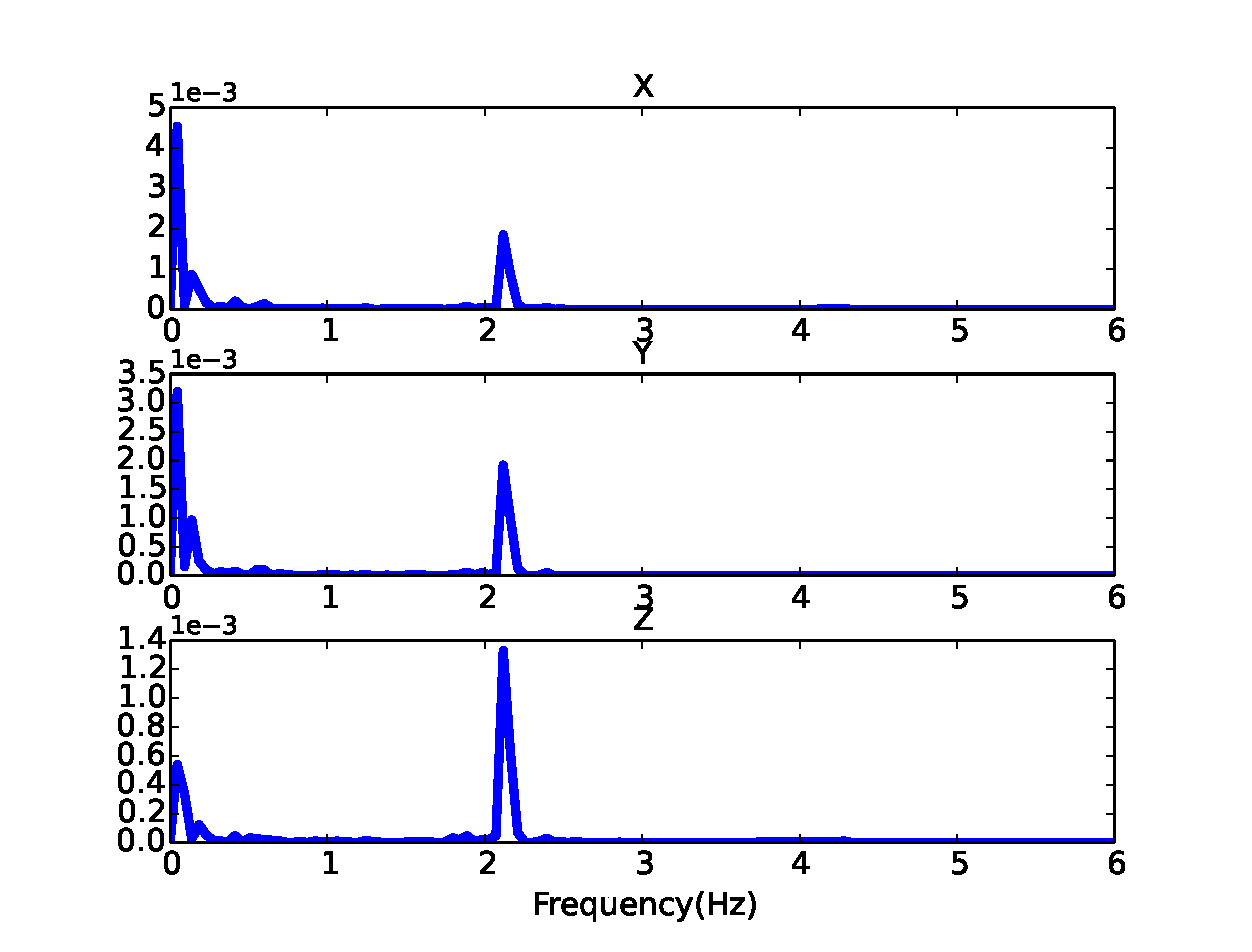
\includegraphics [width=.35\linewidth]{../fig/freq_sub10}&
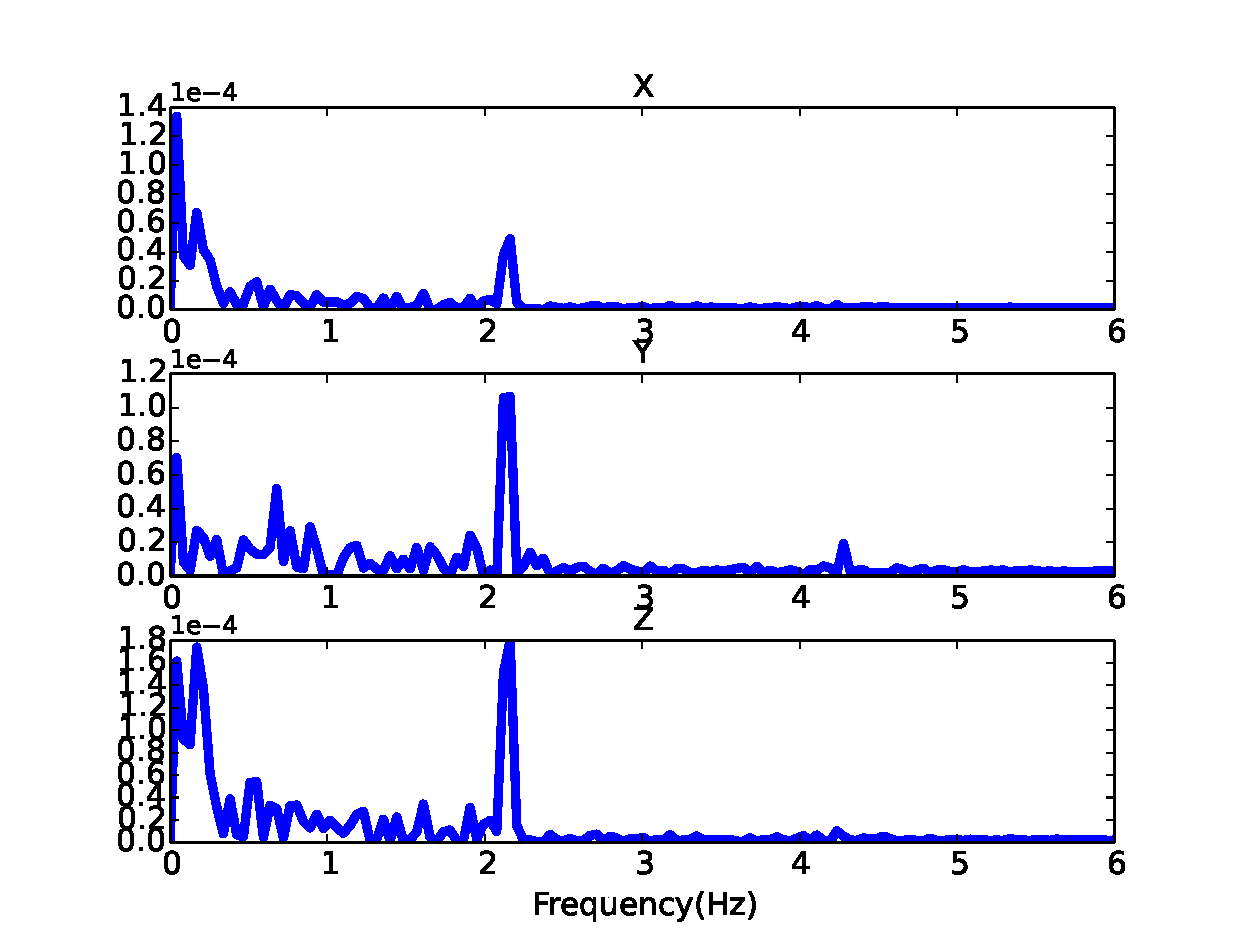
\includegraphics [width=.35\linewidth]{../fig/freq_sub13}\\
(d) User 4& (e) User 5 \\
\end{tabular}
\fi
\end{center}
\caption{\label{fig:raw_freq} Accelerometer data from three users, in the frequency
domain. The data show that the spectrum is significantly
concentrated within 5Hz for all three users.}
\end{figure*}

In this work, we design a system, \systemname, that will enable direct authentication of users to their smart-glass device using
head-movements.  %We envision that our proposed system will be used as an authentication
%interface on the smart-glass wearable device.
The authentication process has two phases: a offline training phase and an 
online authentication phase. In the training phase, the system 
collects the real user's head movement data and use them as 
conducts the training to extract the features. We refer to this set of 
features extracted through the training process as the {\em trained} dataset 
which essentially serves the purpose of a reference in the matching stage. 
In the following discussion, we assume there is only 
one real user for the device for the sake of simplicity. An extension to 
support multiple users per device will be possible with minor modifications, 
namely, by appropriately indexing the users in the trained database.

In the online authentication phase, the sensor readings during the 
authentication attempt are processed, features are extracted, matched with the 
trained set. The user is authenticated upon a successful match.
We posit that \systemname~will run as a service in the device upon power-up, 
similar to the screen-lock in smartphones or the head-nod interface on Google
Glass~\cite{googleglass}.  The authentication process is initiated
by playing a short duration audio track on the device, to which the user 
responds through head-movements. 
Our design is developed based on the idea that humans respond to music 
naturally through head movements, and that such movements are more
significant and unique when the track contains fast beats and/or rhythm.
We will refer to the audio snapshots as {\em music cues} in the rest of the 
paper. 
~\systemname~generates unique features from the head
movements of a user, and uses them as a unique signature for
identifying the right user of the device. The system will
grant access only when the head-movement signature
generated during the login attempt matches with the
original user's signature.

As illustrated in Figure~\ref{fig:sysarch}, the user 
authentication in~\systemname~involves the following key processes:
\begin{itemize}

\vspace{-2pt}\item {\em Sensor data collection}: ~\systemname~records the head-movements
in the form of raw accelerometer signals (in 3 dimensions) using the inbuilt 
accelerometer
sensor on the smart-glass device.
\vspace{-2pt}\item {\em Filtering}: The accelerometer signals are filtered by applying  
a low-pass filter to remove records of extraneous motion.
\vspace{-2pt}\item {\em Signature generation}: The accelerometer signals are
processed through the dynamic-time warping (DTW) tool~\cite{dtw} to obtain a
DTW feature that is treated as the unique signature for the user.
%A user can generate different signatures for different audio tracks. A
%training phase collects the set of signature for each user-audio pair.
\vspace{-2pt}\item {\em Classification}: The signatures are classified as 
a match or not a match, based on a thresholding 
scheme and using the trained data set as a reference. The system grants the 
user access to the device if there is a match 
with sufficient confidence.
%In the former case, the system will grant the user access
%\item {\em Authentication}: The head-movement signature generated  
%during system operation is compared with the original user-audio pair
%signature, and the user is authenticated access if there is a plausible match.
\end{itemize}

%The original signature of the glass user is generated through a
%training phase that is executed when the glass is operated
%by the user for the very first time, and the training data gets
%updated upon each use of the device.
%As shown in Figure~\ref{fig:sysarch} shows the block diagram of
%~\systemname system design.
We will now discuss these design aspects in more detail.
\newpage
\subsection{Sensor Data Collection}
%To facilitate natural head movement, we provide several
%short music tracks with easy-to-follow beats.

The sensor data collection step involves the user wearing
the head-worn device and making head-movements in response to
the music beats played on the device for a stipulated duration of $T$ seconds.
In this duration, the raw accelerometer
signals, from the inbuilt sensor, are collected at
a sampling rate of $r$ samples/sec; the default sampling rate on
Google Glass is 200Hz. The accelerometer data corresponding to one user,  is a 
collection of accelerometer readings on the
3D axis (x, y, and z) collected over $T$ sec duration. 
Figure~\ref{fig:headbanger-illustrate} illustrates the axis 
conventions with respect to the user's head position. 
The data collection unit stores the accelerometer readings in a
matrix with dimensionality $3\times rT$, where each element corresponds
to one signal point. We will refer to this $3\times rT$ as a {\em sample} in 
our design. 
We retain the duration $T$ to be in the order of few seconds, as frequency of 
human head movements are, intuitively, typically in the order of few times per 
second. This intuition will be more clear from the filtering stage to be 
discussed next.
%The sensor data is accumulated in a $30r$ matrix, which we refer to as
%one $ACC$ sample.
%We hypothesize that
%head-movement can serve as a reliable behavioral biometric -- that is, $ACC$
%samples from the same user have smaller distances than samples from different
%users.

\begin{figure*}
\begin{center}
\begin{tabular}{ccc}
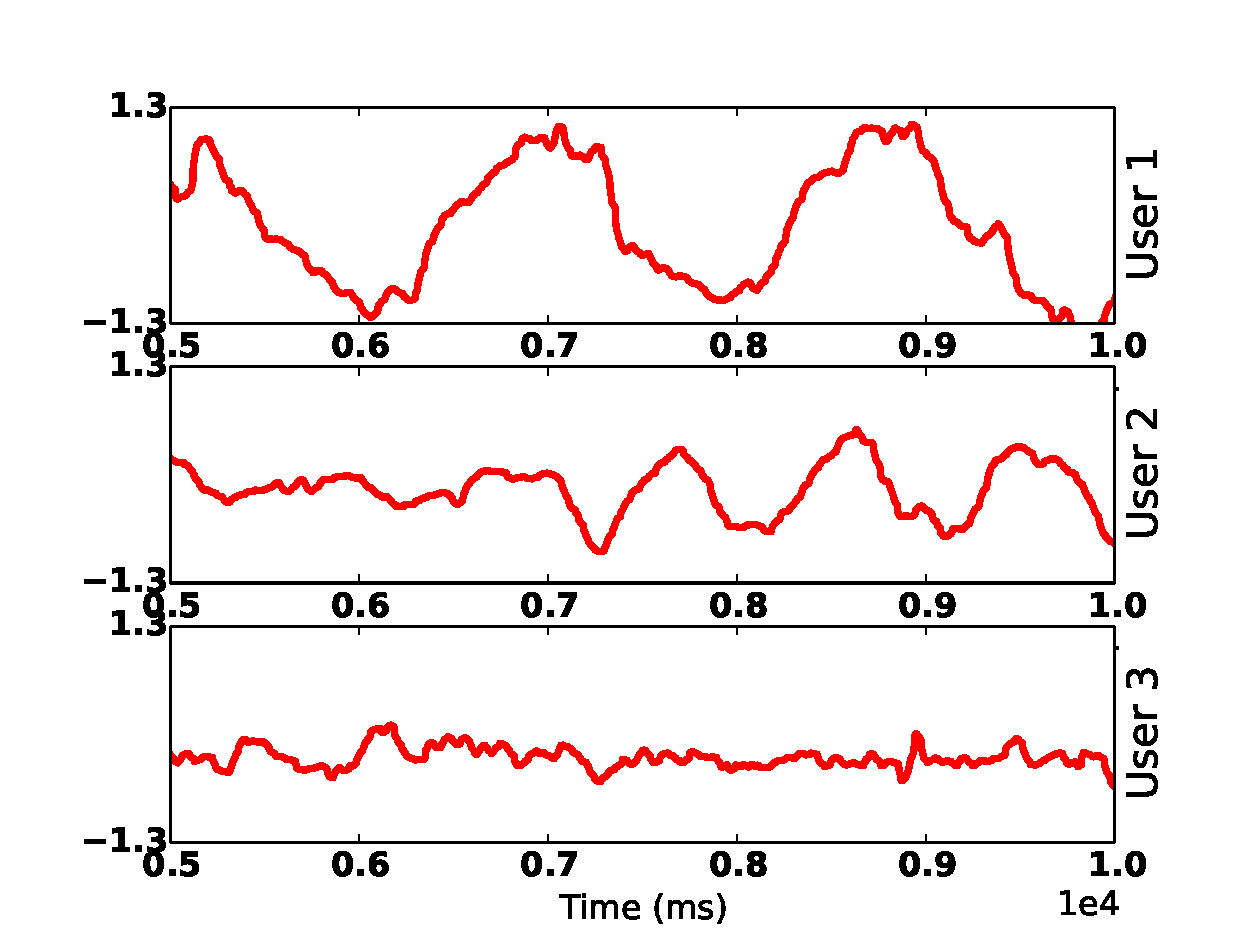
\includegraphics [width=.33\linewidth]{figure/filtered_x.eps}&
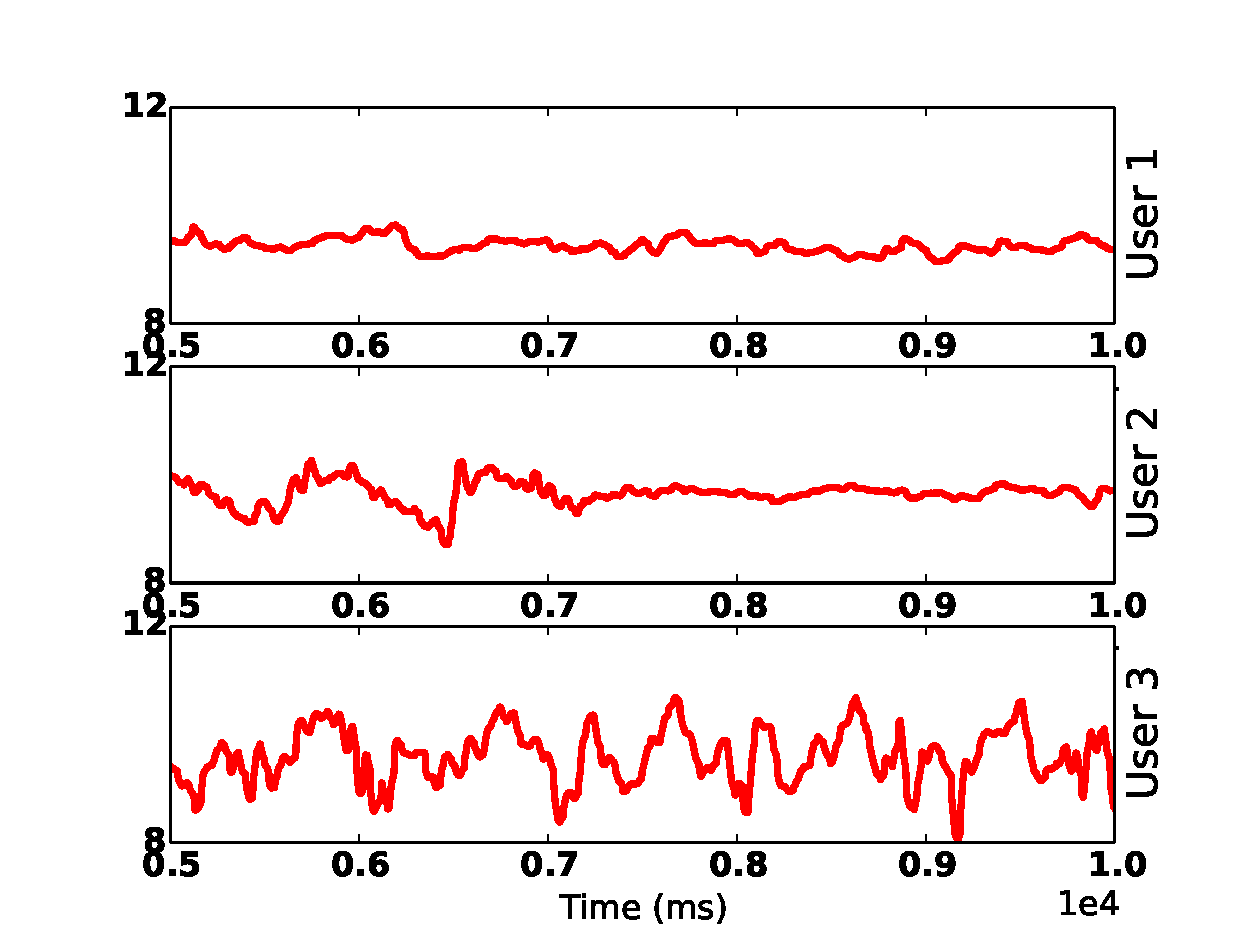
\includegraphics [width=.33\linewidth]{figure/filtered_y.eps}&
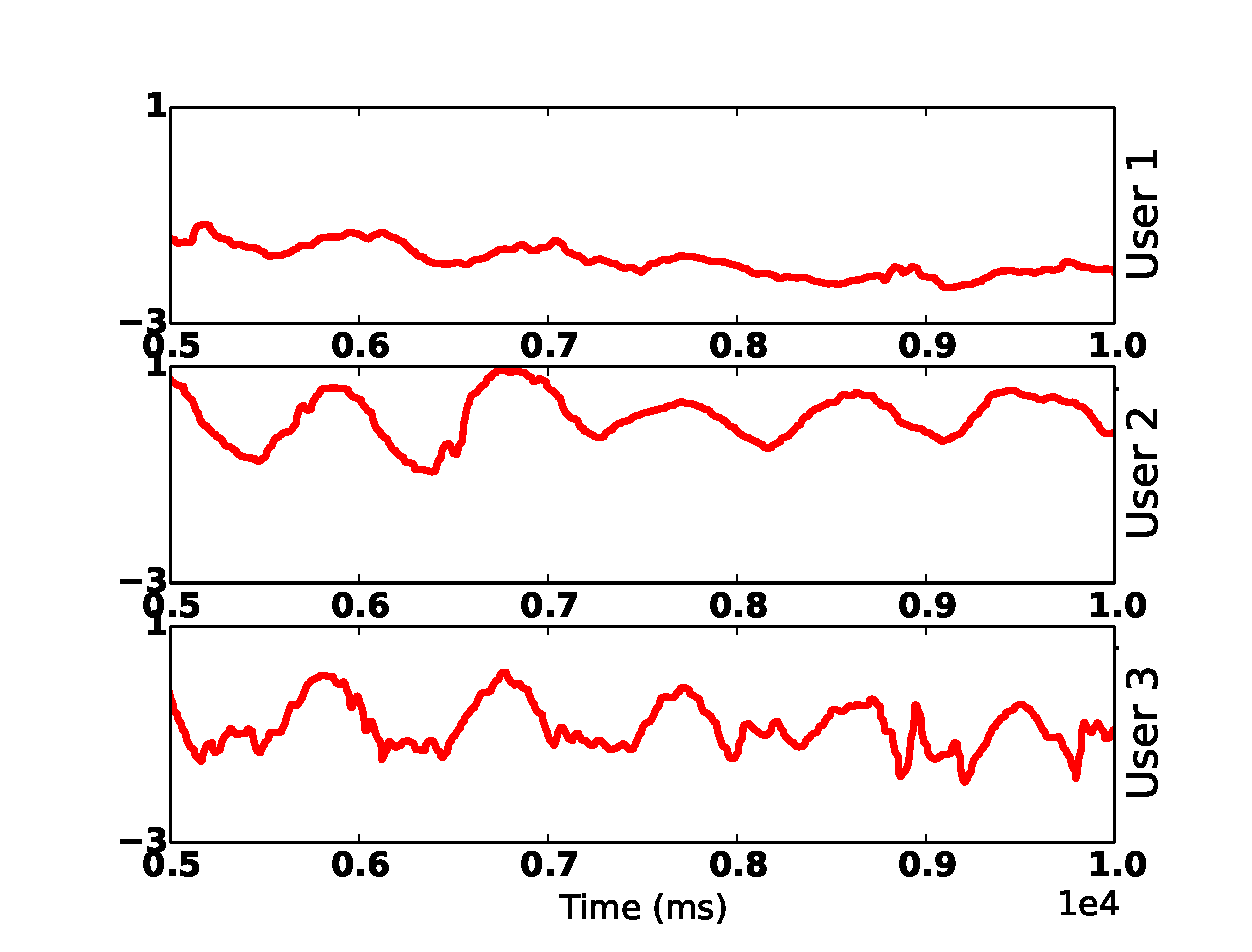
\includegraphics [width=.33\linewidth]{figure/filtered_z.eps}\\
(a) X-Axis & (b) Y-Axis & (c) Z-Axis \\
\end{tabular}

\iffalse
\begin{tabular}{cc}
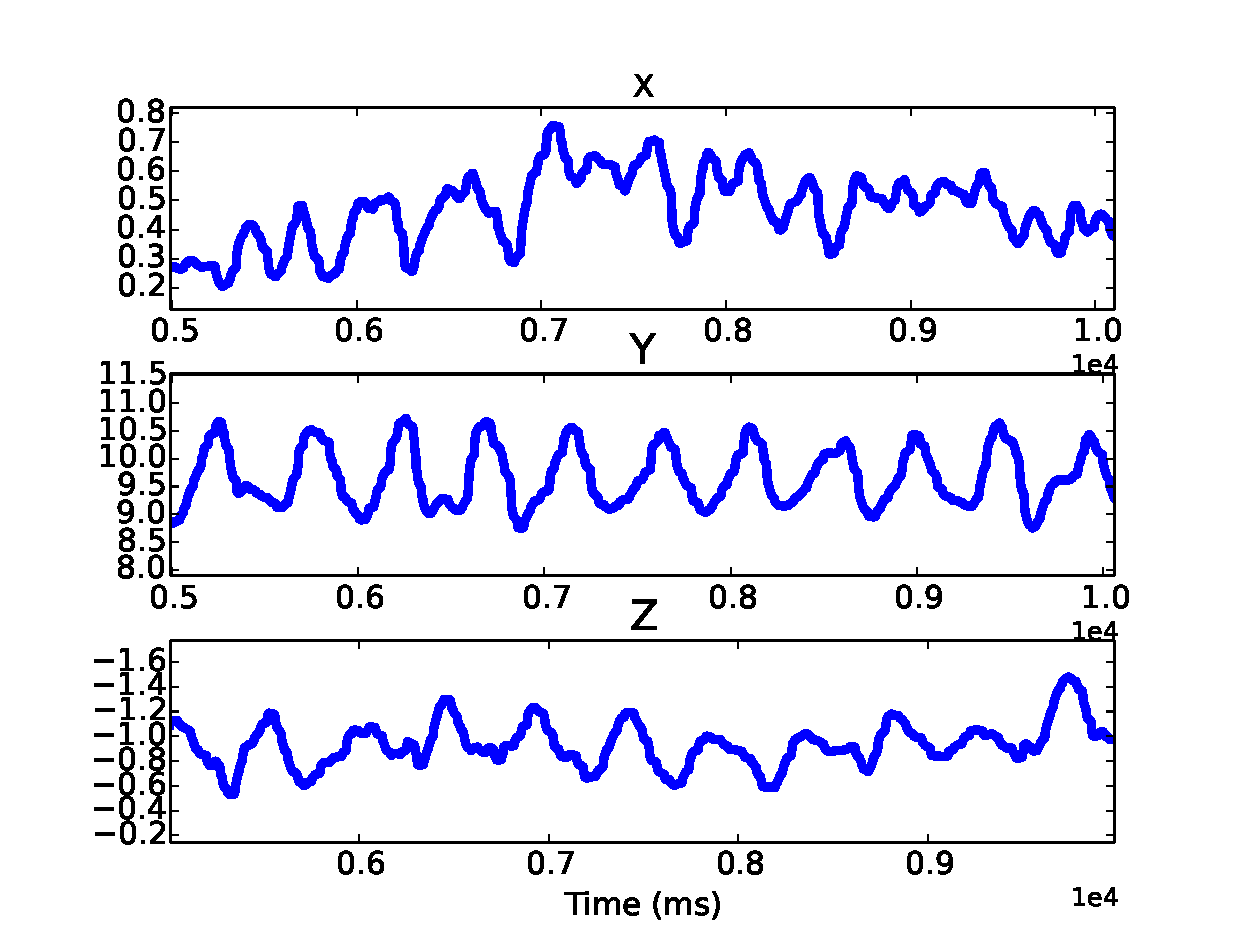
\includegraphics [width=.33\linewidth]{../fig/filer_sub4.eps}&
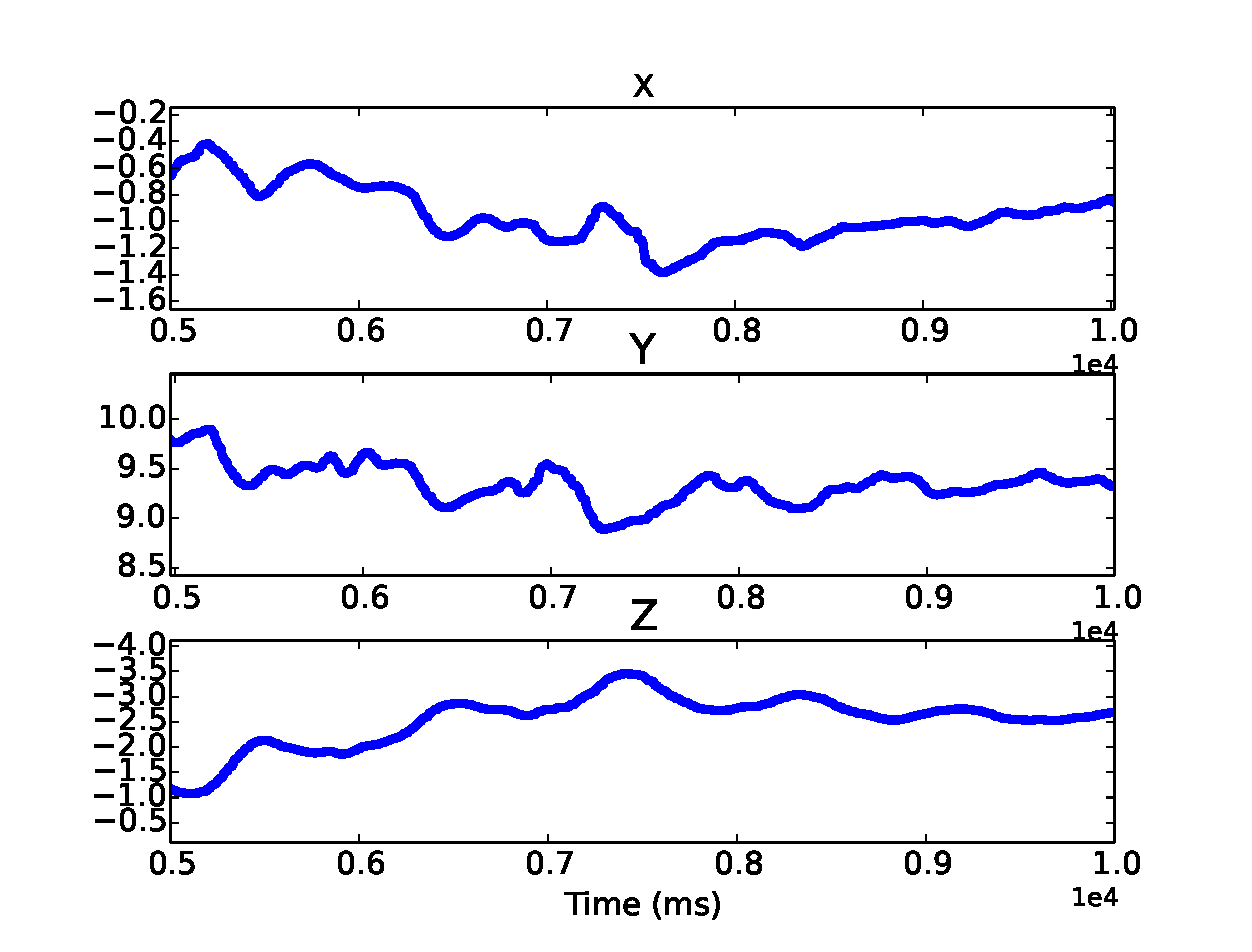
\includegraphics [width=.33\linewidth]{../fig/filer_sub5.eps}\\
(d) User 4& (e) User 5 \\
\end{tabular}
\fi
\end{center}
\caption{Filtered accelerometer signals. Applied Butterworth
filter of order 2 and cut-off frequency 10Hz.
\label{fig:filteredacc}}
\end{figure*}


\subsection{Filtering}

The accelerometer samples are cleaned-up from noise (accelerometer
readings due to spurious movements such as vibrations) through
a filtering stage.
The filtering ensures that the head-movement signature
generated from the accelerometer readings encompasses
only head movements, and not any spurious signals caused due to
vibration or shaking. From the frequency
spectrum of each accelerometer sample, as shown in 
Figure~\ref{fig:raw_freq} 
for three users, we can observe that the spectrum is significantly
concentrated within 5Hz.
We note that music tracks with high tempo, or fast beats, typically contain
beats in the order of the order of hundred beats per minute.
In particular, the high tempo music that we used in our experimentation was 
contained 94 beats per minute~\cite{beats}.
We infer that the head-movement, in response
to the beats, will be of the same order. Hence, we hypothesize that
the signal spectrum in [0,5] Hz range encompass
human head movements; where 0 Hz can indicate that the head is
steady still, and 5 Hz can correspond to a vigorous head-shake.
We filter accelerometer samples using a low-pass digital Butterworth
filter~\cite{challis1983design}. We set a relaxed cut-off frequency of 10Hz.
Even with the relaxed cut-off, the filtering results in
clean accelerometer samples with head-movement patterns
that are prominent and detectable. 
Figures~\ref{fig:filteredacc} (a)-(c) show the filtered results of the raw accelerometer 
samples shown in 
Figure~\ref{fig:raw}; 
compared to raw data, the filtered results are much more 
suitable for subsequent processing.

%\begin{figure}[t]
%\centering
%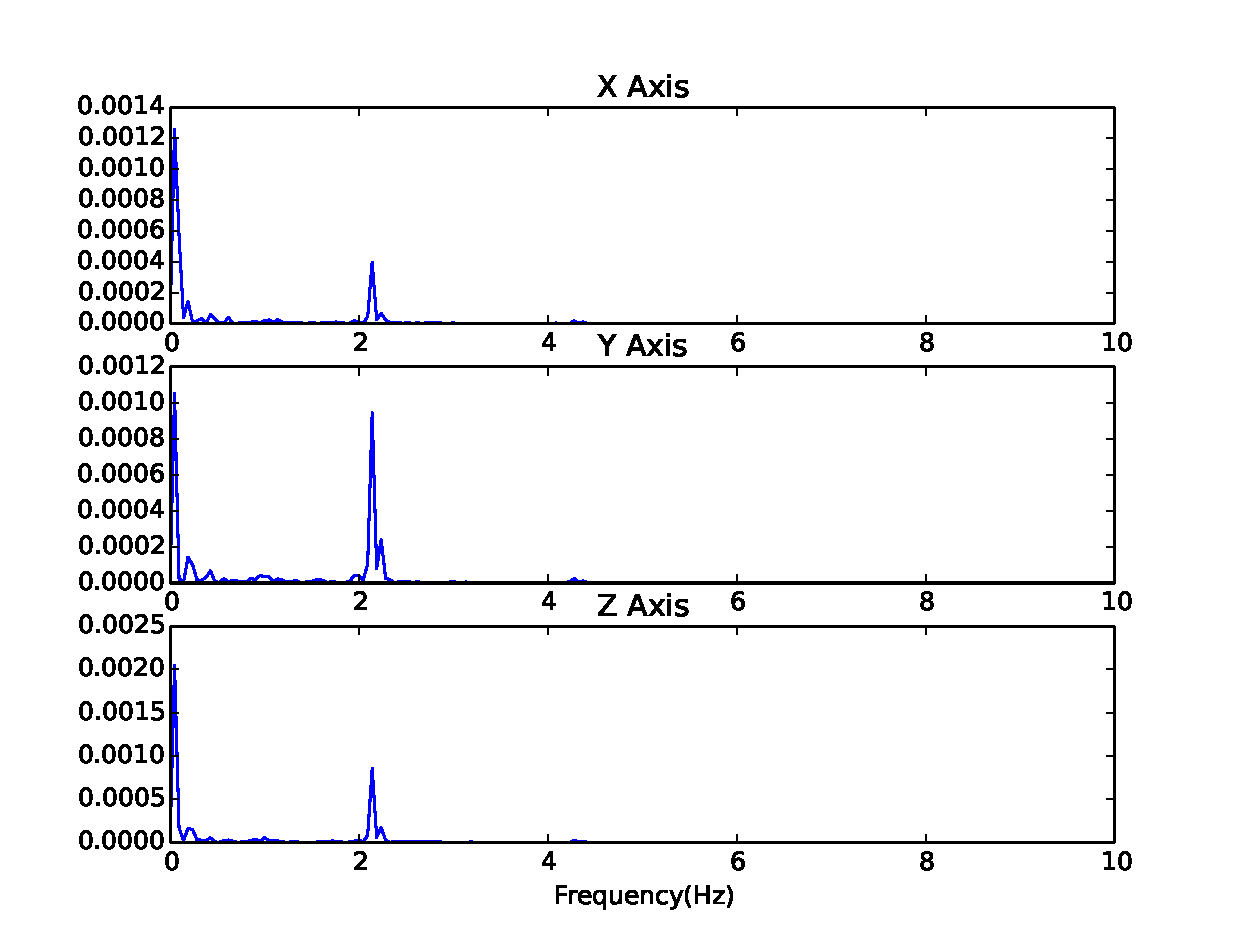
\includegraphics [width=.95\linewidth]{fig/freq_resp.eps}
%\caption{\label{fig:freq_resp}Fiver users' $ACC$ samples in frequency domain.}
%\end{figure}

\subsection{Signature generation}
%\subsection{Quantifying Sample Similarity}

We generate a signature from the accelerometer signals using the
dynamic-time warping (DTW) tool~\cite{dtw}. DTW is generally used
as a similarity matching tool for time-domain analysis of
temporally varying signals.
DTW compares a temporal signal with a reference (temporal) signal over a 
certain time-window and yields a distance measure as the score. A low score 
(DTW distance) implies that the test signal is in close match with the 
reference.
We use the DTW to generate a signature for the head-movements
from the accelerometer signal.
We observed from our preliminary tests that, users often
start head movement at an angle with the vertical which varies among users.
However, we also observed that the head-movements that follow exhibit a 
consistent, and often periodic, patterns over time.
%We empirically observed that the accelerometer signal patterns
%are consistent after the first 1sec duration of head-movements.
Treating the accelerometer sample set from the first trial as a reference, we
apply the DTW algorithm on the successive accelerometer sample set to obtain a
distance score vector, $\hat{d} = (d_x, d_y, d_z)$; the three elements in
$\hat{d}$ denote the DTW distance score in the $x, y, z$ axes, respectively.
By computing the mean of the distance scores obtained for each accelerometer
pair we generate the mean-value DTW distance, which is treated as the
head-movement signature or unique {\em feature} for that particular user and 
audio
combination.

In the offline training phase, we conduct 
%For evaluation purposes, we conduct an elaborate training phase where
$M$ trials of head-movement exercises, collect $M$ training samples, and 
obtain $M-1$ reference distance vectors. We observed from our evaluations (to 
be discussed in the next section) that $M = 30$ can yield in high accuracy 
while $M = 10$ can yield reasonable accuracy. The trade off is the computation 
overhead that goes into conducting the training (primarily DTW computations) 
for the $M$ samples.
%In real usage of the application, 
%the user would conduct only
%two trials of $T$ duration each where trial 1 is treated as reference.
%In this way, the training can be done in-situ. The training data-set is
%updated upon each usage of the authentication interface.
%%Small distance values DTW is expected to return relatively small distance
%%values for samples from the same user, while returning large distance values
%%for samples from different users (that have different movement patterns).
%%Here, $S1$ is the reference

\iffalse
Next we investigate how we can accurately quantify the similarity level
between two accelerometer samples, whose results will be used to classify the users.
After testing various methods,
We decide to adopt the Dynamic Time Warping (DTW) algorithm that is
often used to measure similarity between two waves based on temporal
stimulation.  Unlike many other algorithms, DTW measures the similarity
between two signals that are similar but with phase difference, which is well
suited for our study. In our study, users often start head movement at a
different angle, but exhibit similar, often periodic, pattern for a similar
amount of time. Applying the DTW algorithm on two accelerometer samples $S1, S2$, we
get a vector $(d_x, d_y, d_z)$ denoting the distance in the $x, y, z$ axes
respectively. DTW is expected to return relatively small distance values for
samples from the same user, while returning large distance values for samples
from different users (that have different movement patterns).

YZ: Sugang, we need some detailed equations or algorithms here.
\fi

\subsection{Classification}
%\subsection{Classifying Users}
The classification step labels a test sample based upon the pre-established training/reference samples.
%the trained data-set, DTW signatures (distance
%vector), for each user-audio pair to its corresponding user.
%The classification step essentially separates ambiguous and spoofed
%authentication signatures from the original and generates a database
%of signatures for each user-device-audio pair. We will refer to this database
%as {\em trained signatures} for the rest of the paper.
%
%In this work, we consider an adaptive thresholding strategy. 
%\begin{itemize}
%\item {\em Supervised learning (SVM)}, which generates the trained signatures
%for each user based on a training set that includes the user's original
%signature as well as a number of other false signatures, that do not
%correspond to the user.
%\item {\em Adaptive thresholding}, 
%which generates the trained signatures for each user based on the signatures generated from a select set of trials of the
%same user.

%\end{itemize}
\iffalse
We will now discuss these two methods in more detail.

\subsubsection{SVM-Based Classification}
The SVM based classification goes through the following steps:
\begin{enumerate}
\item Construct the training set by including both ``true'' samples,
corresponding to the device owner, and ``false'' samples, corresponding to the
signatures from random users.
\item Calculate the DTW vectors between any two true samples (with the
resulting DTW vectors referred to as $DTW_{T\rightarrow T}$), as well as DTW
vectors between any true sample and false sample (with the resulting DTW
vectors referred to as $DTW_{T\rightarrow F}$).
\item Given a test sample $S$, calculate the
DTW vectors between $S$ and any true sample (with the resulting vectors
referred to as $DTW_{S\rightarrow T}$) as well as DTW vectors between $S$ and
false samples (with the resulting vectors referred to as $DTW_{S\rightarrow
F}$).
\item Input both, training DTW vectors (i.e., $DTW_{T\rightarrow T}$ \&
$DTW_{T\rightarrow F}$) and test DTW vectors (i.e., $DTW_{S\rightarrow T}$
\& $DTW_{S\rightarrow F}$) to a binary SVM classifier that labels each
signature with a $1$ or $0$ along with an identity corresponding to the
user-audio pair; a $1$ meaning the signature belongs to the right owner and
$0$ that it does not.
\end{enumerate}

{\bf Optimized SVM.} In order to minimize the computing overhead in the above
process and make it suitable for running on a smart-glass, we conduct the SVM
classification in an optimized fashion:
instead of looking at every single training sample from a user, we choose a
small set of representative samples and use them for classification.
Here, we define a user's representative samples as those that
are the most similar to samples from other trials (of the same user). Let us suppose a user's
entire training set has $N$ samples (from $N$ trials). For every sample, we
compute its distance to each of the $N-1$ samples using DTW. Then we choose
the $K$ samples that have the lowest $K$ average distance to the rest of the
training set. By setting an appropriate threshold $K$, we find the
representative samples from the training set. We refer to these $K$ samples as
top $K$ samples of the user. If we choose a small $K$ value, say 3 as opposed
to 20, the computing overhead can be significantly reduced. We conduct this
optimization strategy keeping in mind the increasing latency of SVMs with
training set size. We note to the reader that such an optimization is
only effective when the unoptimized training data-set size is sufficiently
large. %However, such a training data-set collection is a one-time procedure,
%while the top $K$ representative set is updated upon each login attempt of the
%user.
%For example, in our experiments, we use a unoptimized training set of
%size 10. In reality, however, we do not expect the user to generate
%signatures
%from 10 trials. Instead, we propose that the signatures
Eqn.~\ref{eq:top1} shows how we calculate the top 1 sample from $N$ samples
from a user.

\begin{eqnarray}
DTW_\mu & = &\frac{\sum_{i\neq{n}}DTW_i(n)}{N}\nonumber\\
DTW_{min} & = &min\{DTW_{\mu 1},...,DTW_{\mu N}\}
\label{eq:top1}
\end{eqnarray}

%In the testing phase, given a testing sample, we calculate its distance to each training set's top $K$ samples. Suppose we have $K$ true training samples, and $fK$ false training sets ($f$ is the number of false training sets), then we will have $(f+1)K$ distance values for the testing sample. We then input these distance values to the SVM classifier which will return the classification result -- $1$ means the user is classified as the owner while $o$ means the user is not classified as the owner.


\subsubsection{Adaptive thresholding-Based Classification}
\fi
%Through empirical trials we observed that the SVM classification may not be very
%robust against false training signatures that come very close to the true
%samples. While finding optimal binary SVM classifier parameters or using a
%multi-class SVM~\cite{weston1999support} are probable solutions, we felt that these
%approaches will add significant overheads to the already complex SVM.
In this study, we developed a simple yet effective classification scheme based on adaptive thresholds. We highlight the aspects of the adaptive thresholding procedure as follows:

\begin{enumerate}

\item Given $M$ training samples, we identify the top $K$ samples that have 
the lowest $K$ average distance to the rest of the
training set, and calculate their DTW vectors to the rest of the samples in 
the training set to obtain $(M-1)K$ distance vectors. We call this resultant 
vector as Top-$K$ reference distance vector. For example, if $K = 1$, then we 
call the resulting algorithm as Top-1 algorithm; if $K \neq 1$, then we call 
the resulting algorithm as Top-$K$ voting algorithm.
The voting refers to the procedure that the DTW computation results for each 
sample in the training set is referenced, sorted (in increasing order of DTW 
scores) and the classification (a binary index, match or no-match) is 
performed on the top $K$ entries. The final classification result corresponds 
to the majority vote from the list of $K$ results.
By using top $K$ samples, instead of all $M$ samples in the training set, we 
significantly reduce the computation overhead in the authentication 
process. In our evaluation, we will study the impact of $K$ value; in 
particular, we evaluate for $K = 1$ and $K = 3$.

\item Compute the 3 element (x,y,z axis) mean $\mu$ vector and standard
deviation $\sigma$ vector of the top-$K$ distance vector, for each 
authentication trial.
We define ``true'' range as $[\mu-n\sigma, \mu+n\sigma]$, where $n$ is a design
parameter that will be fixed by the designer. The samples outside this
range are labeled as ``false''.
We refer to this range $[\mu-n\sigma, \mu+n\sigma]$ as the threshold in our
classifier design, and the strictness of this threshold is characterized by 
the value of $n$; a large $n$ relaxes the threshold but can increase the false 
acceptance rate while a strict threshold with small $n$ value can result in a 
high rejection rate of true samples. In our system we aim to reach an optimal 
value of $n$ that can result in acceptable accuracy. 
%\item Steps (1) to (3) are repeated when a new sample set is added to the
%training database resulting in an updated threshold. This way, the thresholding
%based classification is adaptive to the user trials. As we will show in our
%evaluations, the thresholding approach is more robust than the SVM approach,
%through both yield reasonable authentication accuracy.
\end{enumerate}
If the user's data is classified as ``true'' then the user is authenticated to the device; otherwise, the user is rejected. 


\iffalse
\subsection{Authentication}

The authentication step results in a binary output that corresponds to
either allowing or disallowing the user to unlock the device.
In this paper, we make two reasonable assumptions pertaining to authentication
on the smart-glass device: (i) homogeneity of
accelerometer sensors for all smart-glasses (from a particular vendor), and (ii)
that the device is registered to the user with an associated PIN or passcode,
and that the head-movement signature is used for secondary verification.
Upon entry of the correct password, the device verifies the identity
of the user based on the head-movement signature.

In the head-movement authentication phase, given a test sample, we classify the sample as true (1) or false
(0) based on one of the two classifiers discussed above. If the result is true, the user is accepted; otherwise
the user is rejected.
\fi

%The authentication mechanism for each of the two classification strategies are
%as follows:

%{\bf SVM.} Given a test sample, classify the sample as true (1) or false
%(0) based on the SVM classifier. %If the result is true, compute the euclidean
%distance between the each of the top $K$ true signatures and the classified
%test signature. If the euclidean distance is below a pre-set threshold
%(obtained empirically from training phase)


%{\bf Adaptive thresholding.} Given a testing sample, calculate the
%DTW distance between the testing sample and the top $K$ representative
%samples. If the resulting distance mean falls within threshold range, then the
%result is ALLOW USER; otherwise, the user is rejected.
